% Tao: Temporarily put the 3-in-1 screenshot here. Please move it to the proper place.
\begin{figure*}[ht]
\centering
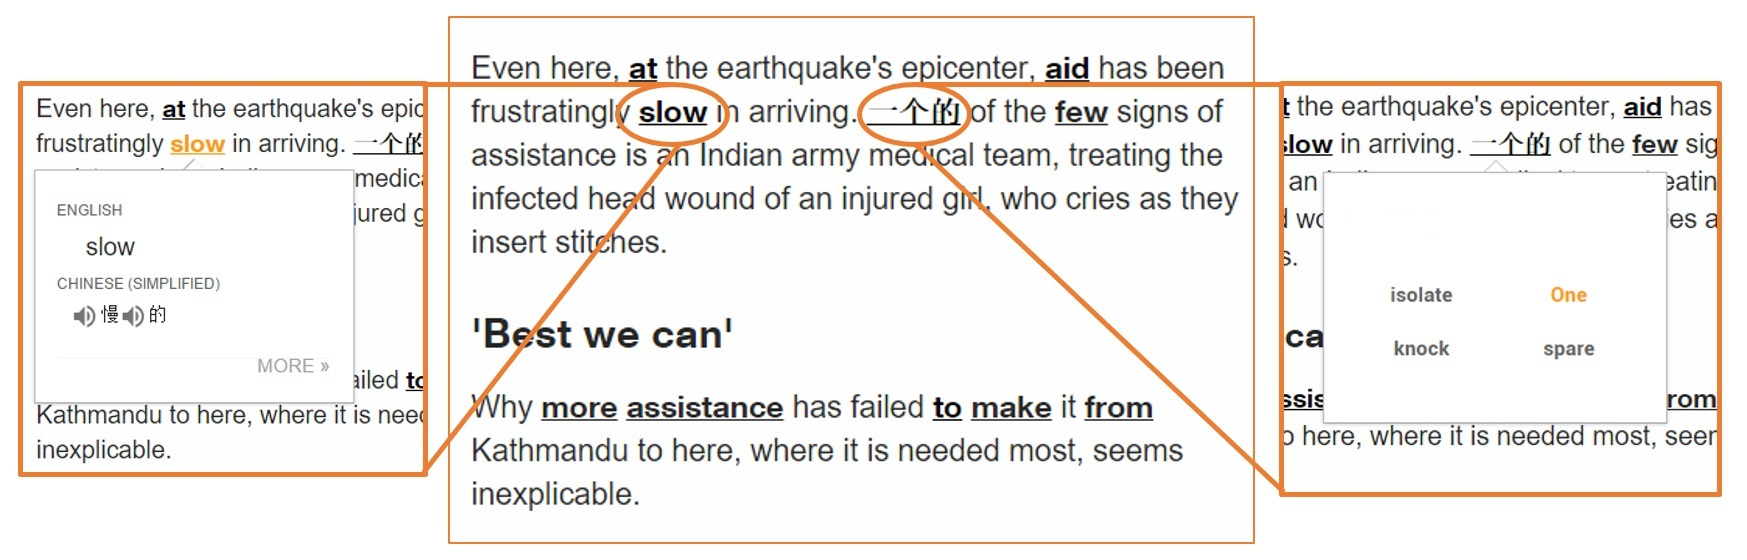
\includegraphics[width=0.99\textwidth]{chrome_extension.jpg}
\caption{Merged screenshots of our Chrome extension on the CNN English
  article {\it Treacherous journey to epicenter of deadly Nepal
    earthquake}.  Underlined components are clickable to yield
  tooltips of two different forms: (l) a definition for learning, (r)
  a multiple-choice interactive test.}
\label{fig:chrome_extension_1}
\end{figure*}

\section{The {\tt SystemA} Chrome Extension}
%%Muthu: To introduce and motivate context here
% Tao: Please also mention our bilinguial dictionary 

\begin{CJK}{UTF8}{gbsn}
We give a running scenario to illustrate the use of our language
learning platform, {\tt SystemA}.  When a learner browses to an
English webpage on a news website, our extension selectively replaces
certain original English words with their Chinese translation
(Figure~\ref{fig:chrome_extension_1}, middle).  While the meaning of
the Chinese word is often apparent in context, the learner can choose
to learn more about the replaced word, by mousing over the translation
to reveal a definition tooltip (Figure~\ref{fig:chrome_extension_1},
left) to aid mastery of the Chinese word.  Once the learner has
encountered the replaced word a few times, {\tt SystemA} will assess
the learner's mastery by generating a multiple choice translation test
on the target word (Figure~\ref{fig:chrome_extension_1}, right). Our
learning platform thus can be viewed as three logical use cases:
{\it translating}, {\it learning} and {\it testing}. \\

%% \begin{figure}[ht]
%%   \centering
%%   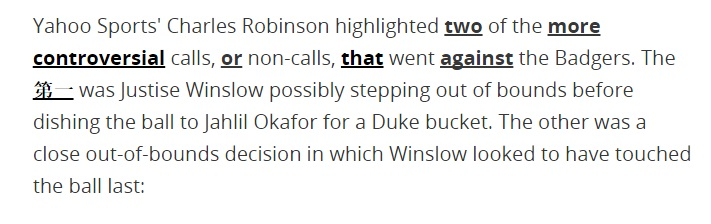
\includegraphics[width=0.45\textwidth]{software_design_2.jpg}
%%   \caption{Screen shot of Translating Component}
%%   \label{fig:software_design_2}
%% \end{figure}
{\bf Translating.}  We pass the main content of the webpage from the
extension client to our server for candidate selection and
translation.  As certain words are polysemous, the server must select
the most appropriate translation among all possible meanings. Our
initial selection method replaces any instance of words stored in our
dictionary. For translation, we check the word's stored meanings
against the machine translation of each sentence obtained from the
Microsoft Bing Translation API (hereafter, ``Bing'').  Matches are
deemed as correct translations and are pushed back to the Chrome
client for rendering.

%% \begin{figure}[ht]
%%   \centering
%%     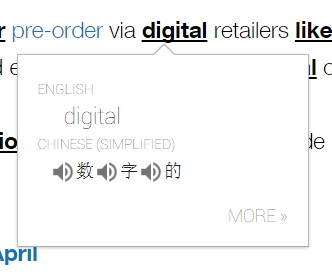
\includegraphics[width=0.3\textwidth]{software_design_4.jpg}
%%   \caption{Screen shot of popover with highlighted English word}
%%   \label{fig:software_design_4}
%% \end{figure}
%%  \begin{figure}[ht]
%%      \centering
%%     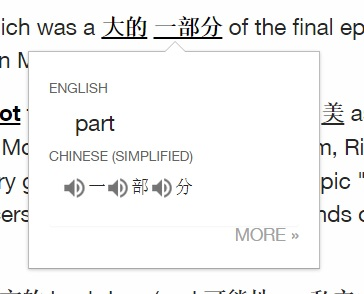
\includegraphics[width=0.3\textwidth]{software_design_5.jpg}
%%      \caption{Screen shot of popover with highlighted Chinese word}
%%      \label{fig:software_design_5}
%%  \end{figure}

{\bf Learning.} Hovering the mouse over the replacement Chinese word
causes a tooltip to appear, which gives the translation,
pronunciation, simplified and traditional written form, and a {\tt
  More} link that loads additional contextual example sentences (that
were previously translated by the backend) for the learner to study.
The more link must be clicked for activation, as we find this
two-click architecture helps to minimize latency and the loading of
unnecessary data.  The server keeps record of the learning tooltip
activations, logging the enclosing webpage URL, the target word and
the user identity.
% Min: doesn't seem to be shown, actually.  Where is an example sentence?
%  Figure \ref{fig:software_design_5} is the screen
% shot of the pop over with its example sentences.

%% \begin{figure}[ht]
%% \centering
%%   \centering
%%   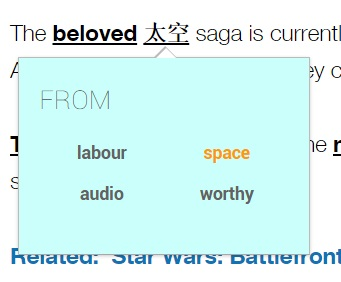
\includegraphics[width=0.3\textwidth]{software_design_7.jpg}
%%   \caption{Screenshot of English test popover}
%%   \label{fig:software_design_7}
%% \end{figure}
%% \begin{figure}[ht]
%%     \centering
%%   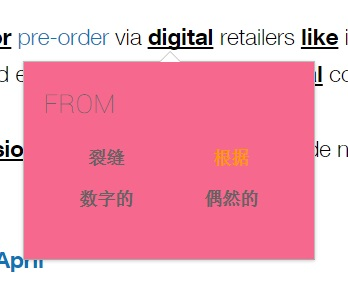
\includegraphics[width=0.3\textwidth]{software_design_8.jpg}
%%   \caption{Screen shot of Chinese test popover}
%%   \label{fig:software_design_8}
%% \end{figure}

{\bf Testing.}  After the learner encounters the same word a
pre-defined number $t=3$ times, {\tt SystemA} generates a MCQ test
to assess mastery.  When the learner hovers over the replaced word,
the test is shown for the learner to select the correct answer. When
an option is clicked, the server logs the selection, and the correct
answer is revealed by the client extension.  Statistics on the user's
test history are also updated.

%{\bf Classifying words category.}
% Tao: please keep the label, as I have referred it in wsd section
% Min: will note and change
\subsection{News Categories}
\label{subsec:category}
As our learning platform is active only on certain news websites, we
model the news category of both individual words and webpages. Of
particular importance to {\tt SystemA} is the association of words to a
news category, which is used downstream in both word sense
disambiguation (Section~\ref{sec:wsd}) and the generation of
distractors in the interactive tests (Section~\ref{sec:distractor}).
Here, our goal is to automatically find highly relevant words to a
particular news category -- e.g., ``what are typical {\it finance}
words?''.  

We first obtain a large sample of categorized English news webpages,
by creating custom crawlers for specific news websites.  We use a seed
list of words that are matched against a target webpage's URL.  If any
match, the webpage is deemed to be of that category.  For example, a
webpage that has the seed word ``football'' in its URL is deemed of
category ``Sports''.  However, note that Chinese news sites have a
different categorization scheme, and as such, we first had to manually
align the different categories based on our observation (See
Table~\ref{table:cat}).  After a survey of a number of English and
Chinese news websites, we decided on seven categories: namely,
``World'', ``Technology'', ``Sports'', ``Entertainment'', ``Finance'',
``Health'' and ``Travel''.
 
% Tao: As we discussed, need to mention the category alighment of English and Chinese news and show the example words in a table?

\begin{table}[ht]
\centering
  \caption{News Category Alignment between English and Chinese.}
  \label{table:cat}
  \begin{tabular}{| p{2.3cm} | p{2.0cm} | p{1.8cm} |}
    \hline
    {\bf English \qquad Category} & {\bf Chinese \qquad Category} & {\bf Example Words}\\
    \hline
    Entertainment & Entertainment & ``superstar"\\
    \hline
     World &  Military, \qquad International, Social & ``attacks'' \\
    \hline
    Finance & Finance & ``investment"\\
    \hline
    Sports & Sports & ``score'' \\
    \hline
    Fashion &  Lady & ``jewelry"\\
    \hline
    Travel  & Auto & ``natural''\\
    \hline
   Health &  & ``stress'' \\
    \hline
  \end{tabular}
\end{table}


We tokenize and part-of-speech tag the main body text of the
categorized articles, discarding punctuation and stopwords.  For
Chinese, we additionally carried out Chinese word segmentation using
the Stanford Chinese word segmenter. The remaining words are
classified to a news category based on document frequency. A word $w$
is classified to a category $c$ if it appears a tunable threshold
$\delta=10$ more often than its average category document frequency.
Note that a word can be categorized to multiple categories under this
scheme.


%% A word w is classified into category C(i) if it satisfies Equation~\ref{equation:Distractor_3}::

%% \begin{equation}
%% f (w, C(i)) - sw(w)/n >= \delta
%% \label{equation:Distractor_3} 
%% \end{equation}  

%% The confidence factor $\delta$ can be a positive integer between 0 and the average number of articles in each category. It means on average, the word w must appear in a specific category C(i) $\delta$ times more than it appear in other category before it can be classified into category C(i).

%% It is obvious that a higher confidence factor value will result in less number words getting classified, but it will result in getting words that are more accurate. A suitable confident value is selected to generating category-related words in the later section.



\end{CJK}

